\documentclass[a4paper]{article}

%% Language and font encodings
\usepackage[english]{babel}
\usepackage[utf8x]{inputenc}
\usepackage[T1]{fontenc}

%% Sets page size and margins
\usepackage[a4paper,top=2cm,bottom=2cm,left=2cm,right=2cm,marginparwidth=1.75cm]{geometry}

%% Sets row spaces
\usepackage{setspace}
\renewcommand{\baselinestretch}{1.0}

%% packages for tables
\usepackage{booktabs}

%% Useful packages
\usepackage{amsmath}
\usepackage{graphicx}
\usepackage[colorinlistoftodos]{todonotes}
\usepackage[colorlinks=true, allcolors=blue]{hyperref}
\usepackage[numbers,sort&compress]{natbib} 
\usepackage{float}	% used for fix the location of tables and graphics
\usepackage{subfigure}  % multi-pictures in the same line
\newcommand{\upcite}[1]{\textsuperscript{\cite{#1}}}
\newcommand{\topcaption}{%
	\setlength{\abovecaptionskip}{0pt}%
	\setlength{\belowcaptionskip}{10pt}%
	\caption}

%_____________________________________________

\title{\textbf{Numerical Methods Solving ODE}}
\author{
	Ye, Fengyang (3180111549) \\
	Tang, Yuan (3180111524)   \\
	Du, Yiqing (3180112696)   \\
	Shu, Yue (3180111518)     \\
	Li, Ruiqi (3180111638)
}

\begin{document}
	
	\maketitle
	
	%_____________________________________________
	\section{Introduction}
	
	At present, Ordinary Differential Equation (ODE) has been widely used in many aspects such as physics, biology and economics. In practical problems, it is particularly important to find the solution of ordinary differential equations. Despite the analytical solution can find the accurate answer, in some practical problems either it is hard to find the analytic solutions or the solving process is too complicated. In this case, it is extremely important to find the numerical solution of ODE by some methods (such as Euler method, Runge-Kutta method and Adams method). In this report, several methods -- Euler method, Runge-Kutta method and Adams method—have been compared in the process of solving the two practical problems.
	
	%_____________________________________________
	
	\subsection{Euler’s Method}
	
	Euler’s method approximates the value of $\Phi(t)$ in the region $[t_n, t_{n+1}]$ of the curve by a straight line. In this report we mainly talk about four methods—the Forward Euler’s Method, the Backward Euler’s Method, the Trapezium Euler’s Method and the Improved Euler’s Method.
	
	The Forward Euler’s Method approximate the original curve with a tangent line of slope $f(t_n, y_n)$. The formula is in the form:
	
	\begin{equation}\label{eq.1}
		y_{n+1} = y_n + hf(t_n, y_n), \enspace n = 0,1,2,...
	\end{equation}
	
	The Backward Euler’s Method approximate the original curve with a tangent line of slope $f(t_{n+1}, y_{n+1})$. The formula is in the form:
	
	\begin{equation}\label{eq.2}
		y_{n+1} = y_n + hf(t_{n+1}, y_{n+1}), \enspace n = 0,1,2,...
	\end{equation}	
	
	The Trapezium Euler’s Method approximate the original curve with a tangent line of slope ${1/over2}(f(t_n )+f(t_(n+1)))$. The formula is in the form:
	
		\begin{equation}\label{eq.1}
		y_{n+1} = y_n + {h\over2}(f(t_n )+f(t_(n+1))), \enspace n = 0,1,2,...
	\end{equation}
	
	The Improved Euler’s Method combines the Forward Euler’s Method and the Trapezium Euler Method. The formula is in the form:
	
	\begin{equation}\label{eq.3}
		y_{n+1} = y_n + \frac{f_n + f(t_n + h, y_n + hf(t_n, y_n))}{2}h, \enspace, n = 0,1,2,...
	\end{equation}	

	%_____________________________________________
	
	\subsection{The Runge-Kutta Method}
	
	The Runge-Kutta Method is similar to the Euler’s Method, however, in this method, we try to find the slope with a few more points on the region $[t_n, t_{n+1}]$, then taking a weighted average of the slope values at these points, and using the resulting value as the approximate slope $k$.
	In this report we discuss the third-order three-stage Runge-Kutta method and fourth-order four-stage Runge-Kutta method. The formula of third-order three-stage Runge-Kutta method is in the form:
	
	\begin{equation}\label{eq.4}
		y_{n+1} = y_n + h(\frac{k_{n1} + 4k_{n2} + k_{n3} }{6}), \enspace n = 0, 1, 2,...
	\end{equation}

	Where
	
	\begin{align} \nonumber
		k_{n1} &= f(t_n, y_n), \\ \nonumber
		k_{n2} &= f(t_n + {1 \over 2}h, y_n + {1 \over 2}hk_{n1}), \\ \nonumber
		k_{n3} &= f(t_n + h, y_n - hk_{n1} + {1 \over 2}hk_{n2}), \\ \nonumber
	\end{align}
	
	The formula of fourth-order four-stage Runge-Kutta method is in the form:
	
		\begin{equation}\label{eq.4}
		y_{n+1} = y_n + h(\frac{k_{n1} + 2k_{n2} + 2k_{n3} + k_{n4} }{6}), \enspace n = 0, 1, 2,...
	\end{equation}

	Where
	
	\begin{align} \nonumber
		k_{n1} &= f(t_n, y_n), \\ \nonumber
		k_{n2} &= f(t_n + {1 \over 2}h, y_n + {1 \over 2}hk_{n1}), \\ \nonumber
		k_{n3} &= f(t_n + {1 \over 2}h, y_n + {1 \over 2}hk_{n2}), \\ \nonumber
		k_{n4} &= f(t_n + h, y_n + hk_{n3}), \\ \nonumber
	\end{align}
	
	%_____________________________________________
	
	\subsection{Adam’s Method}
	
	Adam’s Method makes use of a polynomial $P_k(t)$ of degree $k$ to approximate $phi'(t)$ and evaluates the integral of $phi'(t)$.
	Second-order Adams-Bashforth formula is
	
	\begin{equation}\label{eq.6}
		y_{n+1} = y_n + {3 \over 2}hf_n - {1 \over 2}f_{n-1}, \  n = 0,1,2,...
	\end{equation}
	
	Fourth-order Adams-Bashforth formula is
	
	\begin{equation}\label{eq.7}
		y_{n+1} = y_n + {h \over 24}(55f_n - 59f_{n-1} + 37f_{n-2} - 9f_{n-3}), \  n = 0,1,2,...
	\end{equation}
	
	Adams-Moulton formulas is
	
	\begin{equation}\label{eq.7}
		y_{n+1} = y_n + {h \over 24}(9f_{n+1} + 19f_{n} - 5f_{n-1} + f_{n-2}), \  n = 0,1,2,...
	\end{equation}
	
	
	
	%_____________________________________________
	
% 	\section{Analytical Solution}
	
% 	\subsection{Problem 1}
	
% 	Before using numerical methods to calculate, we try to use analytical methods to calculate the accurate answer.
% 	Substitute $y(t) = \sum_{n=0}^{\infty} a_n t^n$ into the ODE and equate coefficients. Then we can get
	
% 	\begin{equation}
% 		(n+1)a_{n+1}-a_{n-1} = 
% 			\begin{cases}
% 				\sum_{k=0}^{n-k}, & \text{$n \neq 2$} \\
% 				2a_0a_n + a_1^2 + 1, & \text{$n = 2$}
% 			\end{cases}
% 	\end{equation}

% 	Which is hard to calculate. 
	
% 	%_____________________________________________
	
% 	\subsection{Problem 2}
	
% 	Similar to Problem 1, we calculate analytical solution at first.
% 	We also substitute $y(t) = \sum_{n=0}^{\infty} a_n t^n$ into the ODE.
	
% 	%_____________________________________________
	
	\section{Methods}
	
	\subsection{Problem 1}
	
	For problem 1, we are supposed to compute the solution of such a first-order nonlinear ODE: 
	
	\begin{equation} \label{eq:ode1}
	    y' = y^2 + ty + t^2 \tag{ODE1}
	\end{equation}
	
	\subsubsection{Domain}
	
	First we need to state the ODE113() in MATLAB with a stepsize h=0.0001 as the accurate solution when comparing the error of each method.
	
	To acquire a maximal solution of this problem, an relatively accurate domain should be computed. The estimation of the boundaries can be done both in analytical and numerical way. A pure analytical way can be Taylor Series, which yet is not the point of this report.
	
	At the beginning, some graphic methods could be made use of to provide a big picture of how the system works, e.g. a slope field as \autoref{fig:slope_field1}.
	
	\begin{figure}[H]
		\centering
		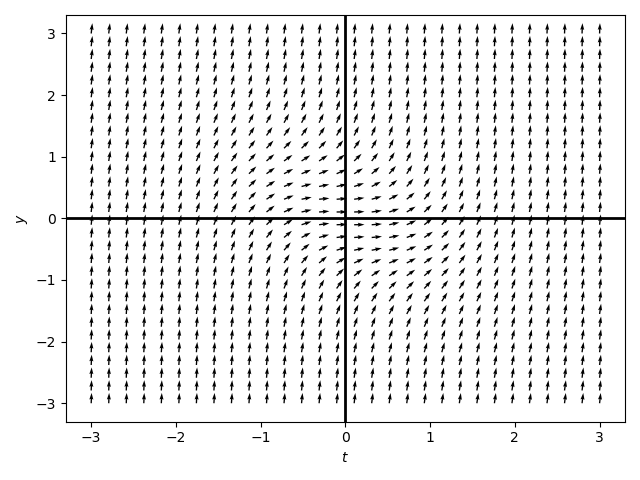
\includegraphics[width=6cm]{img/slope_field1.png}
		\caption{\label{fig:slope_field1} The slope field of $f(t, y)$ of Problem 1}
	\end{figure}
	
	In \autoref{fig:slope_field1} it seems that the solution curve of problem 1 is monotonic increasing. In fact, the derivative $y' = y^2 + ty + t^2 = (y + {1 \over 2}t)^2 + {3 \over 4}t^2 \geq 0$, thus it's globally increasing.
	
    Also, \autoref{fig:slope_field1} turns out that the maximal solution might be restricted between two vertical asymptotes. Therefore determining the domain is to determine these two essential asymptotes, and at this moment a using numerical method to make some attempts can be helpful.
    
    We make use of three numerical methods, i.e. the Euler Improved Method, the Runge-Kutta Method ($4^{th}$ order) and the Adams-Monlton Method to determine the value of $t$ when $y$ is infinity.
    
    \begin{table}[H]
    \centering
    \resizebox{280pt}{!}{%
    \begin{tabular}{@{}lllllll@{}}
    \toprule
    \multicolumn{1}{l}{}           & \multicolumn{2}{c}{\textbf{Euler improved}}                       & \multicolumn{2}{c}{\textbf{RK 4th}}                               & \multicolumn{2}{c}{\textbf{Adams-Monlton}}      \\ \midrule
    \multicolumn{1}{l}{\textbf{$h$}} & \multicolumn{1}{l}{\textbf{$a_1$}} & \multicolumn{1}{l}{\textbf{$b_1$}} & \multicolumn{1}{l}{\textbf{$a_1$}} & \multicolumn{1}{l}{\textbf{$b_1$}} & \multicolumn{1}{l}{\textbf{$a_1$}} & \multicolumn{1}{l}{\textbf{$b_1$}} \\ \hline
    0.01                           & -2.17                           & 0.91                            & -2.14                           & 0.88                            & -2.12                  & 0.85                   \\
    0.005                          & -2.15                           & 0.885                           & -2.13                           & 0.87                            & -2.1201                & 0.855                  \\
    0.001                          & -2.126                          & 0.864                           & -2.123                          & 0.861                           & -2.1202                & 0.858                  \\
    0.0005                         & -2.1235                         & 0.8615                          & -2.122                          & 0.86                            & -2.1205                & 0.8585                 \\
    0.0002                         & -2.1218                         & 0.86                            & -2.121                          & 0.8594                          & -2.1206                & 0.8587                 \\
    0.0001                         & -2.1212                         & 0.8594                          & -2.1209                         & 0.8591                          & -2.1207                & 0.8588                 \\ \bottomrule
    \end{tabular}%
    }
    \caption{Determine t When y is infinity}
    \label{tab:ivp1_inf_1}
    \end{table}
    
	It seems that the left bound of the solution is around $a_1 = -2.12$ and the right around $b_1 = 0.85$. To be more accurate, some analytical approaches should be adopted. 
	
	We will use two functions $f_1$ and $f_2$ to squeeze $f$ and reduce the range. The sign relationship between t and y should be determined first. We use the numerical results of the Adams-Monlton method at $t = -2.120$ and $t = 0.858$ in \autoref{tab:adams-monlton-domain-1} to illustrate some details.
	
    \begin{table}[H]
    \centering
    \resizebox{200pt}{!}{%
    \begin{tabular}{@{}lll@{}}
    \toprule
    \multicolumn{1}{l}{}           & \textbf{$t = -2.120$} & \textbf{$t = 0.858$} \\ \midrule
    \multicolumn{1}{l}{\textbf{$h$}} & \textbf{$y$}          & \textbf{$y$}         \\ \hline
    0.01                           & -\infty               & \infty           \\
    0.005                          & -\infty               & \infty           \\
    0.001                          & -\infty               & \infty           \\
    0.0005                         & -1657.12353516        & 1177.64002010    \\
    0.0002                         & -1523.43140641        & 1142.81318658     \\
    0.0001                         & -1518.10313846         & 1141.29183391   \\ \bottomrule
    \end{tabular}%
    }
    \caption{y of the results of the Adams-Monlton method when t = -2.120 and t = 0.858}
    \label{tab:adams-monlton-domain-1}
    \end{table}
    
    It's obvious that $t$ and $y$ have the same sign, plus the monotonicity and $|y| > |t|$ near the boundary, we can have such relationship: $y^2 < y^2 + ty + t^2 < 3y^2$. Therefore we obtain two solvable ODEs $y' = f_1(t, y) = y^2$ and $y' = f_2(t, y) = 3y^2$ to locate the boundary accurately. By solving these two ODEs we obtain:
    
    \begin{align}
        \Phi_1(t) &= -\frac{1}{t + C_1} \\
        \Phi_2(t) &= -\frac{1}{3t + C_2}
    \end{align}
    
    For the left boundary, we substitude the initial problem with $y(-2.120) = -1518.10313846$ from the results of \autoref{tab:adams-monlton-domain-1} and obtain $C_1 = 2.12065871$ and $C_2 = 6.36065871$, which turns out that the left bound should be restricted between $-2.12065871$ and $-2.12021957$, i.e., $-2.12065871 < a_1 < -2.12021957$.
    
    For the right boundary, similarly, we take the initial problem as $y(0.858) = 1141.29183391$ and obtain $C_1 = -0.85887620$ and $C_2 = -2.57487620$, which turns out that the right boundary should locate between $0.85829206$ and $0.85887620$, i.e., $0.85829206 < b_1 < 0.85887620$. 
	
	In conclusion, the domain of the solution of problem 1 is:
	
	$$
	\left\{
    	\begin{aligned}
    	    t &\in (a_1, b_1) \nonumber \\
    	    a_1 &\in (-2.12065871, -2.12021957) \nonumber \\
    	    b_1 &\in (0.85829206, 0.85887620) \nonumber
    	\end{aligned}
	\right.
	$$
	
	%______________________________________________
	
	%% TODO: The beginning of error analysis?
	When t is a point not close to the vertical asymptote, at h=0.0001, all methods have very small error. (see Appendix) When the value of t is near vertical asymptote, for all methods, even at small h, their error is much larger. Therefore, it is hard to compare which methods have smaller error just looking through percentage errors near vertical asymptote. \\
	
	We can estimate that there might be two vertical asymptotes, $a_1$, $b_1$. Since the slope of the vector tends to be infinity near $t=-2$ and $t=1$, so we can have a try: let $a_1$ very close to -2 and $b_1$ very close to 1 to find accurate vertical asymptotes.
	
	\begin{table}[H]
		\centering
		\resizebox{400}{!}{%
			\begin{tabular}{@{}ccccccccc@{}}
				\toprule
				& \multicolumn{2}{c}{\textbf{Euler Implicit}} & \multicolumn{2}{c}{\textbf{Euler Explicit}} & \multicolumn{2}{c}{\textbf{Euler Improved}} & \multicolumn{2}{c}{\textbf{Euler Trapezium}} \\ \midrule
				\textbf{$h$} & \textbf{$a_1$}          & \textbf{$b_1$}          & \textbf{$a_1$}          & \textbf{$b_1$}          & \textbf{$a_1$}          & \textbf{$b_1$}          & \textbf{$a_1$}           & \textbf{$b_1$}          \\
				\hline 
				0.01       & -2.07                & 0.82                 & -2.26                & 1                    & -2.17                & 0.91                 & -2.11                 & 0.85                 \\
				0.005      & -2.09                & 0.83                 & -2.195               & 0.935                & -2.15                & 0.885                & -2.115                & 0.855                \\
				0.001      & -2.115               & 0.853                & -2.137               & 0.875                & -2.126               & 0.864                & -2.1201               & 0.859                \\
				0.0005     & -2.118               & 0.856                & -2.129               & 0.8675               & -2.1235              & 0.8615               & -2.1206               & 0.8591               \\
				0.0002     & -2.1196              & 0.8578               & -2.1242              & 0.8624               & -2.1218              & 0.86                 & -2.1208               & 0.8592               \\
				0.0001     & -2.1202              & 0.8584               & -2.1225              & 0.8607               & -2.1212              & 0.85964              & -2.1209               & 0.8592               \\ \bottomrule
			\end{tabular}%

		}
	\caption{Using Euler Method to Determine $t$ When $y$ is infinity}
	\label{tab:euler_inf}
	\end{table}

	%____________________________________________
	
	\subsubsection{The Euler Method}

	When $h=0.01$, vertical asymptotes are not stable. As $h$ is decreasing, $a_1$, $b_1$ gradually reach to a stable value. When $h=0.0001$, the value of $a_1$, $b_1$ calculated by these four methods is absolutely close. Digitally, we can solve that $a_1=-2.1212$, $b_1=0.8594$.
	
	%_____________________________________________
	
	\subsubsection{The Runge-Kutta Method}
	
	The stable value of $a_1$, $b_1$ can be got when $h=0.0001$. RK 4th has more accuracy, but in this particular problem, compared with RK 3rd, it doesn’t fully manifest. When $h=0.01$ or $0.005$, the value of $a_1$, $b_1$ is not so accurate, but not far from stable value. Therefore, we can solve $a_1=-2.1209$, $b_1= 0.8591$.
	
	\begin{table}[H]
		\centering
		\resizebox{180pt}{!}{%
			\begin{tabular}{@{}ccccc@{}}
				\toprule
				& \multicolumn{2}{c}{\textbf{RK 3rd}} & \multicolumn{2}{c}{\textbf{RK 4th}} \\ \midrule
				\textbf{h} & \textbf{a1}      & \textbf{b1}      & \textbf{a1}      & \textbf{b1}      \\
				0.01       & -2.15            & 0.89             & -2.14            & 0.88             \\
				0.005      & -2.135           & 0.875            & -2.13            & 0.87             \\
				0.001      & -2.124           & 0.862            & -2.123           & 0.861            \\
				0.0005     & -2.122           & 0.8605           & -2.122           & 0.86             \\
				0.0002     & -2.1212          & 0.8596           & -2.121           & 0.8594           \\
				0.0001     & -2.121           & 0.8592           & -2.1209          & 0.8591           \\ \bottomrule
			\end{tabular}%
		}
		\caption{Using Runge-Kutta Method to Determine t When y is infinity}
		\label{tab:rk_inf}
	\end{table}
	
	%_____________________________________________
	
	\subsubsection{The Adams Method}
	
	For Adams Bashforth method, when $h$ is not small enough, the value of $a_1$, $b_1$ can’t be stable. Just when $h$ is smaller than the level of $10^{-3}$, $a_1$, $b_1$ will tend to be stable. However, for Adams Molton method, no matter what value $h$ is, in other words, for $h=0.01,0.005,0.001,0.0005,0.0002,0.0001$, in each condition, the value of $a_1$, $b_1$ have little difference. So it can be concluded that Adams Monlton has more accuracy than Adams Bashforth. As a result, we can solve $a_1=-2.1207$, $b_1=0.8588$.
	
	\begin{table}[H]
		\centering
		\resizebox{220pt}{!}{%
			\begin{tabular}{@{}ccccc@{}}
				\toprule
				& \multicolumn{2}{c}{\textbf{Adams-Bashforth}} & \multicolumn{2}{c}{\textbf{Adams-Monlton}} \\ \midrule
				\textbf{h} & \textbf{a1}           & \textbf{b1}          & \textbf{a1}          & \textbf{b1}         \\
				\hline
				0.01       & -2.21                 & 0.95                 & -2.12                & 0.85                \\
				0.005      & -2.17                 & 0.905                & -2.1201              & 0.855               \\
				0.001      & -2.13                 & 0.868                & -2.1202              & 0.858               \\
				0.0005     & -2.1255               & 0.8635               & -2.1205              & 0.8585              \\
				0.0002     & -2.1226               & 0.8608               & -2.1206              & 0.8587              \\
				0.0001     & -2.1216               & 0.8598               & -2.1207              & 0.8588              \\ \bottomrule
			\end{tabular}%
		}
		\caption{Using Adams Method to Determine t When y is infinity}
		\label{tab:adams_inf}
	\end{table}

	%_____________________________________________
	\subsubsection{Solution}
	
	Combining the solution graphs using different methods, the solution graph is as \autoref{fig:ivp1_sol}.
	
	\begin{figure}[H]
		\centering
		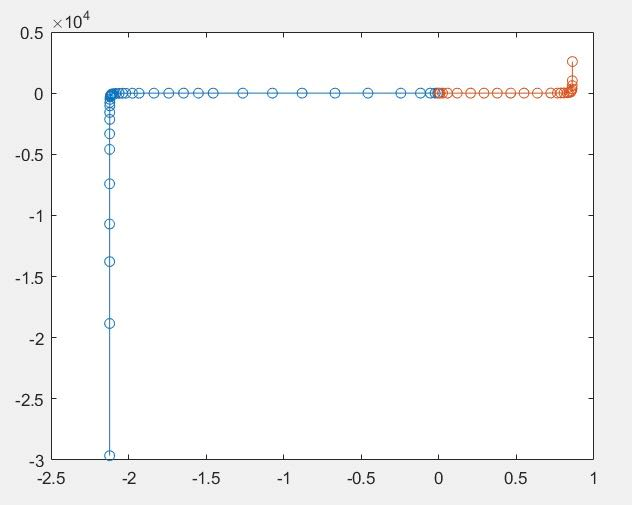
\includegraphics[width=8cm]{img/ivp1_sol.png}
		\caption{\label{fig:ivp1_sol} The Solution of Problem 1}
	\end{figure}

	
	
	
	%_____________________________________________
	
	\subsection{Problem 2}
	
	For problem 2, we are supposed to compute the solution of such a first-order nonlinear ODE: 
	
	\begin{equation} \label{eq:ode2}
	    y' = y^3 + ty^2 + t^2y + t^3 \tag{ODE2}
	\end{equation}
	
	% $y' = y^3 + ty^2 + yt^3 + t^3$
	
	\subsubsection{Domain}
	
	We start with the determination of the domain of solution. Same as problem 1, a slope field can be constructed to help understanding the tendency. According to the slope field \autoref{fig:slope_field2} shown below, the slopes seem not approach to infinite on the left side. Also, it seems that all the points below $y= -t$ have negative slope and all the points upon have positive slope. The numerical results of improved Euler method in \autoref{tab:IVP2_y} also shows the tendency that it approaches to $y = -t$ when $t$ is approaching to negative infinity. 
	
	\begin{figure}[H]
		\centering
		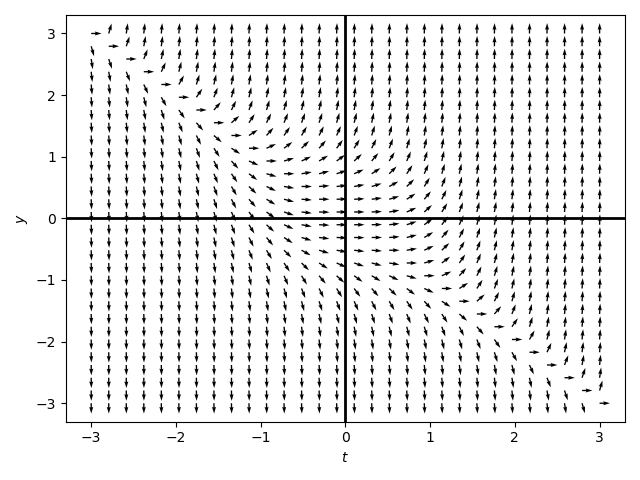
\includegraphics[width=6cm]{img/slope_field2.png}
		\caption{\label{fig:slope_field2} The slope field of $f(t, y)$ of Problem 2}
	\end{figure}
	
    \begin{table}[H]
    \centering
    \resizebox{350pt}{!}{%
    \begin{tabular}{@{}llllllllll@{}}
    \toprule
    \multicolumn{1}{c}{\textbf{t}} & \multicolumn{1}{c}{-50}     & \multicolumn{1}{c}{-45}        & \multicolumn{1}{c}{-40}        & \multicolumn{1}{c}{-35}        & \multicolumn{1}{c}{-30}         & \multicolumn{1}{c}{-25}         \\
    \midrule
    \multicolumn{1}{c}{\textbf{y}} & \multicolumn{1}{c}{49.9998} & \multicolumn{1}{c}{44.9997531} & \multicolumn{1}{c}{39.9996875} & \multicolumn{1}{c}{34.9995918} & \multicolumn{1}{c}{29.99944441} & \multicolumn{1}{c}{24.99919992} \\
     \bottomrule
    \end{tabular}%
    }
    \caption{Using Four Euler Method to Compute y Value}
    \label{tab:IVP2_y}
    \end{table}
    
    This qualitative tendency is proved as follows. Although \autoref{eq:ode2} is not an autonomous system, a "phase space" with $t$ as a parameter can still be constructed, as shown in the left-hand side in \autoref{fig:ivp2_phase}. The graph illustrates that the graph of $y' = f(y)$ has only one zero-crossing at $(-t, 0)$, and points near the line $y \equiv -t$ tend to go away from it (the blue arrows show the tendency), meaning this line is asymptotically unstable. In other words, if we go from $t = 0$ to $t = -\infty$, the sign of the derivative $y' = \frac{dy}{dt}$ should change, i.e. the graph becomes the right-hand side of \autoref{fig:ivp2_phase}, and the line $y \equiv -t$ now becomes an "asymptote". \\
    
    In addition, the solution $\Phi(t)$ with $t \rightarrow -\infty$ will approach to this "asymbptote" from below, i.e., $\Phi(t) < -t$ with $t < \alpha$, where $\alpha$ is the point where the solution curve coincide with the line $y \equiv -t$. It is because $f_2(t, y)$ can be factorized as $y' = (y + t)(y^2 + t^2)$, making it obvious that the derivative of $\Phi(t)$ is negative if $\Phi(t) < -t$, positive if $\Phi(t) > -t$ and zero if $\Phi(t) = -t$. Therefore, the solution curve with $t < \alpha$ is restricted below the line $y \equiv -t$ because $\Phi(t)' < 0$. $t = \alpha$ is a turning point with $\Phi(\alpha)' = 0$ where the curve rises above $y \equiv -t$ since it should go through the initial condition $y(0) = 1$.
    
    \begin{figure}[H]
       \subfigure 
    {
    	\begin{minipage}{9cm}
    	 \centering      
    		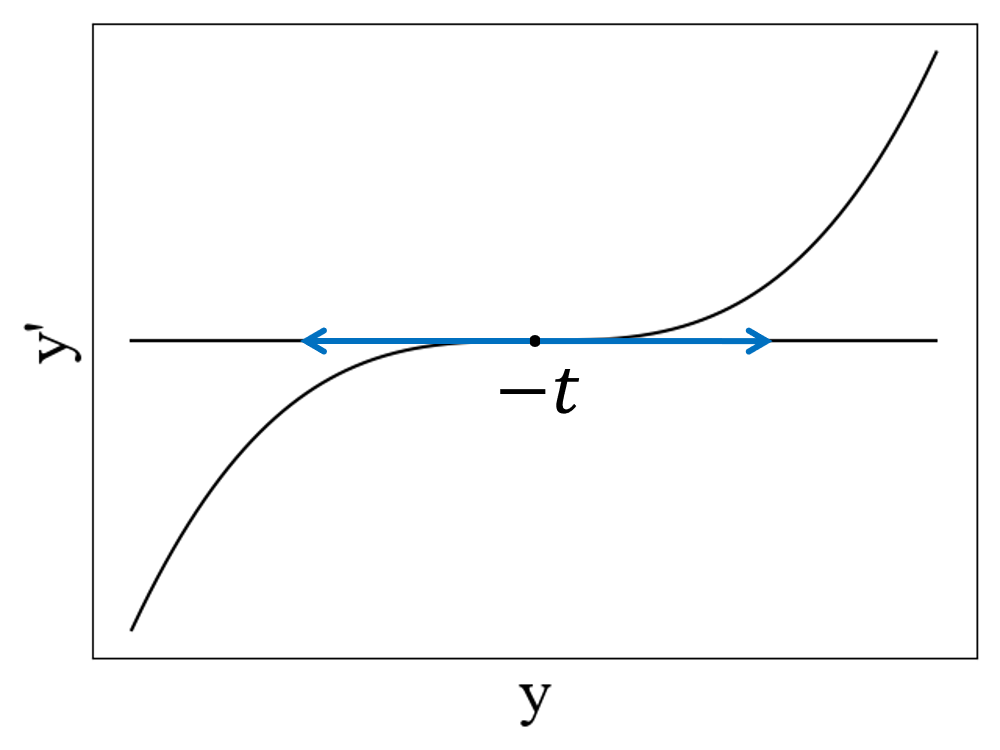
\includegraphics[width=6cm]{img/ivp2_phase_graph_1.png}
    		% \caption{\label{fig:ivp2_phase1}}
    	\end{minipage}
    }
      \subfigure 
    {
    	\begin{minipage}{7cm}
    	\centering      
    		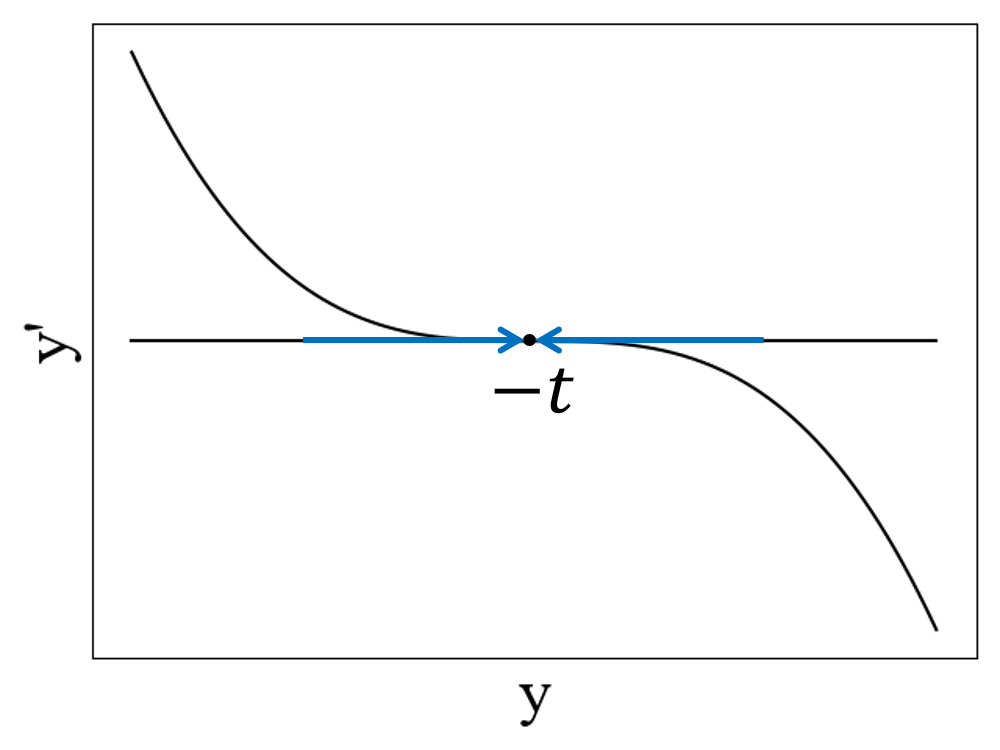
\includegraphics[width=6cm]{img/ivp2_phase_graph_2.png}
    		% \caption{\label{fig:ivp2_phase2} }
    	\end{minipage}
    }
    \caption{\label{fig:ivp2_phase} The phase space of \autoref{eq:ode2}} 
    \end{figure}
    
    Thus, the ODE does not have vertical asymptote on the left side. \\

    For the right vertical asymptote, we use four Euler methods to estimate. The value t is considered as stable location when the change of t value is less than 0.001 by one order step h reduction. The $t$ value where $y$ values first return inf from computation is considered as the approximate location of the vertical asymptote under that condition. Same as problem 1, a table can be constructed as \autoref{tab:IVP2_yinf}.
    
    \begin{table}[H]
    \centering
    \resizebox{400}{!}{%
    \begin{tabular}{@{}llllllllll@{}}
    \toprule
    \textbf{}           & \textbf{Euler\_explicit} & \textbf{Euler\_implicit} & \textbf{Euler\_improved} & \textbf{Euler\_trapezium} \\ 
    \hline
    \textbf{h = 0.01}   & 0.5                      & 0.4                      & 0.48                     & 0.43           \\
    \textbf{h = 0.005}  & 0.495                    & 0.42                     & 0.46                     & 0.435          \\
    \textbf{h = 0.001}  & 0.452                    & 0.436                    & 0.444                    & 0.44           \\ 
    \textbf{h = 0.0005} & 0.446                    & 0.438                    & 0.442                    & 0.4405          \\
    \textbf{h = 0.0002} & 0.4426                   & 0.4392                   & 0.4408                   & 0.4402         \\
    \textbf{h = 0.0001} & 0.4413                   & 0.4396                   & 0.4403                   & 0.4401   \\  
    \bottomrule                                       
    \end{tabular}%
    }
    \caption{Using Four Euler Methods to Compute the Nearest Value t Where y is INF }
    \label{tab:IVP2_yinf}
    \end{table}
 
	According to this numerical result, the difference of t is less than 0.001 when h = 0.0002 in both improved Euler method and trapezium Euler method’s calculation. Thus, t = 0.440 can be considered as the right vertical asymptote location of the ODE if only use the numerical methods. 
	
    \begin{table}[H]
    \centering
    \resizebox{300pt}{!}{%
    \begin{tabular}{@{}lllllll@{}}
    \toprule
    \textbf{h}          & 0.01 & 0.005 & 0.001       & 0.0005      & 0.0002      & 0.0001     \\ 
    \hline
    \textbf{y} & \infty  & \infty   & 25.62721138 & 23.60040387 & 23.43528374 & 23.4279037 \\ 
    \bottomrule
    \end{tabular}%
    }
    \caption{y of the results of the Adams-Monlton method when t = 0.439}
    \label{tab:adams-monlton-domain-2}
    \end{table}
	
	However, analytical approaches similar to problem 1 can still be adopted to acquire more accuracy. To illustrate the details and relationship between $t$ and $y$ we use the Adams-Monlton method at $t = 0.439$ again. Obviously, near the right border $t$ and $y$ are both positive and $y > t$, therefore, we can obtain such an relationship: $y^3 < y^3 + ty^2 +t^2y +t^3 < 4y^3$, which consists of two solvable ODEs $y' = f_1(t, y) = y^3$ and $y' = f_2(t, y) = 4y^3$. By solving them we obtain:
	
	\begin{align}
	    \Phi_1(t) &= \frac{1}{\sqrt{2}\sqrt{C_1 - t}} \\
	    \Phi_2(t) &= \frac{1}{\sqrt{2}\sqrt{C_2 - 4t}}
	\end{align}
	
	Now we can choose one pair of $(t, y)$ from \autoref{tab:adams-monlton-domain-2} as a new initial value. we take $y(0.439) = 23.4279037$ and obtain $C_1 = 0.4399109$ and $C_2 = 1.7569109$, which leads to the results that the right boundary of problem 2 should locate between $0.4392277$ and $0.4399109$, i.e., $0.4392277 < b_2 < 0.4399109$.
	
	In conclusion, the domain of the solution of problem 2 is:
	
	$$
	\left\{
    	\begin{aligned}
    	    t &\in (-\infty, b_2) \nonumber \\
    	    b_2 &\in (0.4392277, 0.4399109) \nonumber
    	\end{aligned}
	\right.
	$$

	%_____________________________________________

     \subsubsection{The Euler Method}

	We define the accurate solution as the result computed by ode113() function in MATLAB with step $h = 0.00001$ for further comparison in the following process. 
	
	We solve the ODE with four different Euler methods, and compute its values with different step h and at $t = 0.25$, $t = 0.30$, $t = 0.35$, $t = 0.40$, which close to its right vertical asymptote.
	
    \begin{table}[H]
    \centering
    \resizebox{\textwidth}{!}{%
    \begin{tabular}{@{}llllllllll@{}}
    \toprule
    \textbf{}         & \multicolumn{4}{c}{\textbf{Euler\_explicit}}           & \multicolumn{4}{c}{\textbf{Euler\_implicit}}            \\ \midrule
    \textbf{h}          & \textbf{t = 0.25} & \textbf{t = 0.3} & \textbf{t = 0.35} & \textbf{t = 0.4} & \textbf{t = 0.25} & \textbf{t = 0.3} & \textbf{t = 0.35} & \textbf{t = 0.4}  \\
    \hline
    \textbf{h = 0.01}   & 1.47770259         & 1.70913766       & 2.09188224        & 2.87954605       & 1.52806345        & 1.8192135       & 2.40057921        & \infty                                                 \\
    \textbf{h = 0.005}  & 1.48930857        & 1.73296161       & 2.14955647       & 3.08663402       & 1.51450889        & 1.78702797       & 2.29743739        & 3.92122702                                                  \\
    \textbf{h = 0.001}  & 1.49920013        & 1.75384897       & 2.20325749        & 3.31926539       & 1.49920013        & 1.75384897       & 2.20903007        & 3.38833119                                                  \\
    \textbf{h = 0.0005} & 1.50047775         & 1.75658869       & 2.21054691         & 3.35489343      & 1.50047775         & 1.75658869       & 2.21054691         & 3.37260573                                                  \\
    \textbf{h = 0.0002} & 1.50124891        & 1.75824716       & 2.21498915        & 3.37718304       & 1.50124891        & 1.75824716       & 2.21498915        & 3.37718304                                                  \\
    \textbf{h = 0.0001} & 1.50150673        & 1.75880245       & 2.21648159        & 3.38477411       & 1.50150673        & 1.75880245       & 2.21648159        & 3.38477411      \\ 
    \midrule
    \textbf{}         & \multicolumn{4}{c}{\textbf{Euler\_improved}}           & \multicolumn{4}{c}{\textbf{Euler\_trapezium}}            \\ \midrule
    \textbf{h}          & \textbf{t = 0.25} & \textbf{t = 0.3} & \textbf{t = 0.35} & \textbf{t = 0.4} & \textbf{t = 0.25} & \textbf{t = 0.3} & \textbf{t = 0.35} & \textbf{t = 0.4}  \\
    \hline
    \textbf{h = 0.01}   & 1.50151241        & 1.75868118       & 2.21550691       & 3.37109489       & 1.50151241        & 1.75911757       & 2.21895347        & 3.41527979                                                \\
    \textbf{h = 0.005}  & 1.50170122        & 1.75918727       & 2.21734767        & 3.38677614       & 1.49778798        & 1.75310181       & 2.20573518        & 3.35601484                                                  \\
    \textbf{h = 0.001}  & 1.50176237        & 1.75935206       & 2.21795425        & 3.39221267       & 1.49920013        & 1.75384897       & 2.20346482        & 3.34431531                                                  \\
    \textbf{h = 0.0005} & 1.5017643         & 1.75935726       & 2.2179735         & 3.3923893       & 1.50047775         & 1.75658869       & 2.21054691         & 3.35929849                                                  \\
    \textbf{h = 0.0002} & 1.50176484        & 1.75935871       & 2.2179789        & 3.392439       & 1.50124891        & 1.75824716       & 2.21498915        & 3.37718304                                                  \\
    \textbf{h = 0.0001} & 1.50176491        & 1.75935892       & 2.21797968        & 3.39244612       & 1.50150673        & 1.75880245       & 2.21648159        & 3.38477411      \\ 
    \bottomrule
    \end{tabular}%
      }
    \caption{Using Four Euler Methods to Compute y Value with different h }
    \label{tab:IVP2_Euler1}
    \end{table}

    Data from the table shows that the solution computed by Improved Euler method is stable when step $h = 0.0005$. Comparing the y values computed by the same method shows that smaller step h leads to higher degree of stability. Therefore, for the other three Euler methods, the solutions could reach the stable condition when it reach a step h which is less than 0.0001. 

    \subsubsection{The Runge-Kutta Method}
    
    We use Runger-Kutta method by 3rd order and 4th order to solve ODE and compute its y values at $t = 0.15$ to $t = 0.35$. 
    
    \begin{table}[H]
    \centering
    \resizebox{\textwidth}{!}{%
    \begin{tabular}{@{}lllllllllllll@{}}
    \toprule
    
    \textbf{}                       & \multicolumn{5}{c}{\textbf{Runge-Kutta\_3rd}}                                                                                                                                                                              & \multicolumn{5}{c}{\textbf{Runge-Kutta\_4th}}                                                                                                               \\ \midrule
    \textbf{h} & \textbf{t = 0.15} & \textbf{t = 0.2} & \textbf{t =0.25} & \textbf{t = 0.3} & \textbf{t = 0.35}   & \textbf{t = 0.15} &\textbf{t = 0.2} & \textbf{t =0.25} & \textbf{t = 0.3} & \textbf{t = 0.35} \\
    \hline
    \textbf{h = 0.01}               & 1.21432129                             & 1.33362603                            & 1.50176378                            & 1.75935475                            & 2.21795648                                                         & 1.21432143                             & 1.33362641                            & 1.50176494                            & 1.75935898       & 2.21797975               \\
    \textbf{h = 0.005}              & 1.21432141                             & 1.33362636                            & 1.50176479                            & 1.75935842                            & 2.2179767                                                           & 1.21432143                             & 1.33362641                            & 1.50176494                            & 1.75935899       & 2.21797993               \\
    \textbf{h = 0.001}              & 1.21432143                             & 1.33362641                            & 1.50176494                            & 1.75935899                            & 2.21797991                                                         & 1.21432143                             & 1.33362641                            & 1.50176494                            & 1.75935899       & 2.21797993               \\
    \textbf{h = 0.0005}             & 1.21432143                             & 1.33362641                            & 1.50176494                            & 1.75935899                            & 2.21797993                                                         & 1.21432143                             & 1.33362641                            & 1.50176494                            & 1.75935899       & 2.21797993               \\
    \textbf{h = 0.0002}             & 1.21432143                & 1.33362641                            & 1.50176494                            & 1.75935899                            & 2.21797993                                                         & 1.21432143                             & 1.33362641                            & 1.50176494                            & 1.75935899       & 2.21797993               \\
    \textbf{h = 0.0001}             & 1.21432143                             & 1.33362641                            & 1.50176494                            & 1.75935899                            & 2.21797993                                                         & 1.21432143                             & 1.33362641                            & 1.50176494                            & 1.75935899       & 2.21797993              \\
    \bottomrule
    \end{tabular}%
    }
    \caption{Using the Runge-Kutta Method by 3rd and 4th order to Compute y Value}
    \label{tab:IVP2_RK}
    \end{table}

    The results at $t = 0.15$ to $0.35$ have been stable at 5th decimal places for 3rd order Runge-Kutta method and 7th decimal places for 4th order one when h is 0.005. It shows that with the same method and the same step h, the higher order computation has higher degree of stability. From the table we could find that the decrease of h also leads to a more stable solution in this method. 
    
    \subsubsection{Adams-Bashforth and Adams-Monlton Method}
    
    The y values determined by the Adams-Bashforth method and Adams-Monlton method are shown in the table below. Adams-Bashforth method reaches stability at 8th decimal places when $h = 0.0002$, and $h = 0.0005$ by Adams-Monlton method. Which shows that Adams-Bashforth method has higher stability than Adams-Monlton in this problem. Compare the result with those from previous methods, it shows that both Adams-Bashforth and Adams-Monlton methods solve the problem better than other methods in stability.
    
    \begin{table}[H]
    \centering
    \resizebox{\textwidth}{!}{%
    \begin{tabular}{@{}lllllllllllll@{}}
    \toprule
     
    \textbf{}                       & \multicolumn{5}{c}{\textbf{Adams\_bashforth}}                                                                                                                                                                       & \multicolumn{5}{c}{\textbf{Adams\_monlton}}                                                                                                          \\ \midrule
    \textbf{h} & \textbf{t = -0.2} & \textbf{t = -0.1} & \textbf{t = 0.1} & \textbf{t = 0.2} & \textbf{t = 0.3} & \textbf{t = -0.2} & \textbf{t = -0.1} & \textbf{t = 0.1} & \textbf{t = 0.2} & \textbf{t = 0.3} \\
    \hline
    \textbf{h = 0.01}               & 0.85718229                             & 0.91666778                             & 1.12500093                            & 1.33361711                            & 1.75925478                                                            & 0.85718192                             & 0.91666752                             & 1.12500238                            & 1.33362721       & 1.75936873                  \\
    \textbf{h = 0.005}              & 0.85718197                             & 0.91666756                             & 1.12500218                            & 1.33362574                            & 1.75935095                                                            & 0.85718192                             & 0.91666752                             & 1.12500238                            & 1.33362646       & 1.75935967                 \\ 
    \textbf{h = 0.001}              & 0.85718197                             & 0.91666756                             & 1.12500218                            & 1.33362641                            & 1.75935899                                                            & 0.85718192                             & 0.91666752                             & 1.12500238                            & 1.33362646       & 1.75935899                  \\
    \textbf{h = 0.0005}             & 0.85718197                             & 0.91666756                             & 1.12500218                            & 1.33362641                            & 1.75935899                                                           & 0.85718192                             & 0.91666752                             & 1.12500238                            & 1.33362646       & 1.75935899                  \\
    \textbf{h = 0.0002}             & 0.85718197                             & 0.91666756                             & 1.12500218                            & 1.33362641                            & 1.75935899                                                            & 0.85718192                             & 0.91666752                             & 1.12500238                            & 1.33362646       & 1.75935899                  \\
    \textbf{h = 0.0001}             & 0.85718197                             & 0.91666756                             & 1.12500218                            & 1.33362641                            & 1.75935899                                                            & 0.85718192                             & 0.91666752                             & 1.12500238                            & 1.33362646       & 1.75935899         \\
    \bottomrule
    \end{tabular}%
    }
    \caption{Using the Adams-Bashforth and Adams-Monlton Method to Compute y Value }
    \label{tab:IVP2_AD}
    \end{table}
    
    \subsubsection{solution}
    Combining the solution graphs using different methods, the solution graph is as
	According to results from the the The accurate solution of problem 2 is shown below.
	
	\begin{figure}[H]
		\centering
		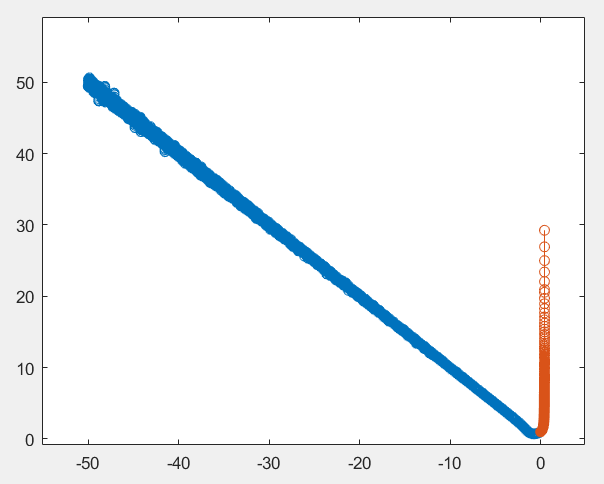
\includegraphics[width=6cm]{img/IVP_2.png}
		\caption{\label{IVP_2} The slope field of $f(t, y)$ of Problem 2}
	\end{figure}
    
%    FIXME OR LEAVEMEALONE
%    \subsubsection{Error Analysis}
        
%    According to the previous result analysis with different methods, Adams-Bashforth method has the highest degree stability among eight methods. For further understanding in the accuracy of the methods, we consider the results computed by each methods with h = 0.001 as stable solutions. We compare the stable solution with the accurate one solved by ode113() function in MATLAB by calculating their average absolute percentage error difference in the domain $[-25,0.44]$. The result is shown below.

%\begin{table}[H]
%\centering
%\resizebox{\textwidth}{!}{%
%\begin{tabular}{@{}lllllllcccccc@{}}
%\toprule
%\textbf{}                      & \multicolumn{3}{c}{\textbf{t = -25}}                                   %                                                               & \multicolumn{3}{c}{\textbf{t = 0.35}}  %                                                                                             \\ \midrule
%\textbf{} & \textbf{y\_stable} & \textbf{y\_ode113()} & \textbf{percentage error} & \textbf{y\_stable} & %\textbf{y\_ode113()} & \textbf{percentage error}             \\
%\hline
%\textbf{Euler Explicit}        & 24.99919992                                        & 25.01208677       %                                   & -0.0515225\%                                   & 2.21648159        %                                 & 2.21136738                                           & 0.2312690\%   %         \\
%\textbf{Euler Implicit}        & 24.99919992                                        & 25.01208677       %                                   & -0.0515225\%                                   & 2.21648159        %                                 & 2.21136738                                           & 0.2312690\%    %                       \\ 
%\textbf{Euler Improved}        & 24.99919992                                        & 25.01208677       %                                   & -0.0515225\%                                   & 2.21797968        %                                 & 2.21136738                                           & 0.2990140\%   %                       \\
%\textbf{Euler Trapezium}       & 24.99919992                                        & 25.01208677       %                                   & -0.0515225\%                                   & 2.21648159        %                                 & 2.21136738                                           & 0.2312690\%   %               \\
%\textbf{RK 3rd}                & 24.99919992                                        & 25.01208677       %                                   & -0.0515225\%                                   & 2.21797993        %                                 & 2.21136738                                           & 0.2990253\%   %                         \\
%\textbf{RK 4th}                & 24.99919992                                        & 25.01208677       %                                   & -0.0515225\%                                   & 2.21797993        %                                 & 2.21136738                                           & 0.2990253\%   %                      \\
%\textbf{Adams Monlton}         & 24.99919992                                        & 25.01208677       %                                   & -0.0515225\%                                   & 2.21797984        %                                 & 2.21136738                                           & 0.2990212\%   %                            \\
%\textbf{Adams Bashforth}       & 24.99919992                                        & 25.01208677       %                                   & -0.0515225\%                                   & 2.21797993        %                                 & 2.21136738                                           & 0.2990253\%   %                            \\
%\bottomrule
%\end{tabular}%
%}
%\caption{percentage error of stable solution and accurate solution at t = -25 and t = 0.35 with h = %0.0001}
%\label{tab:IVP2_error}
%\end{table}
    %FIXME
    %The \autoref{tab:IVP2_error} 
    
	\section{Results}
	Comparing the data and solutions of two questions IVP1 and IVP2, we can find out some typical properties for these methods.
	
	%_____________________________________________
	
	\subsection{Accuracy comparison}
	
   The first conclusion is, for all these methods, the numerical solutions will be more accurate with the step size h decreasing in a certain range. 
   However, the global truncation error of each method is different because of the formula inside. 
   
      
   The second conclusion is the accuracy comparison of different methods. The the error comparison graphs of IVP1, IVP2 are to be made. Since the largest error and smallest error differs largely, we take the errors to the root three times or four times to better compare in one graph. 
   From the first graph of IVP1 below, we can get that the error of Euler explicit method is the  largest. With a h=0.01, the errors of the other four methods are quite similar. 
   For IVP2, the error of Euler explicit method is the largest as well. The Euler improved method has the second largest error. Other methods have quite similar errors.
   All in all, the Adams-Moulton method is the most accurate and the Euler Method has the largest error. The errors of improved Euler method, Euler trapezium method and Runge-Kutta method are quite similar. 
   
   
     %two graphs in same line  
    \begin{figure}[htbp]
    \subfigure 
    {
    	\begin{minipage}{7cm}
    	 \centering      
    		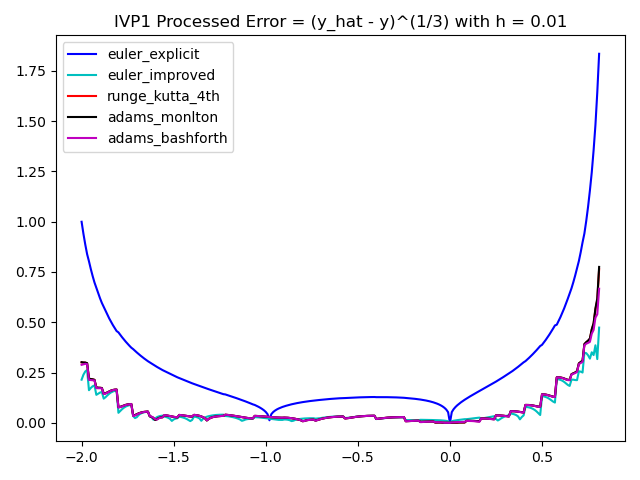
\includegraphics[width=5cm]{img/ivp1_error.png}
    		\caption{\label{fig:ivp1_error} }
    	\end{minipage}
    }
    \subfigure 
    {
    	\begin{minipage}{7cm}
    	\centering      
    		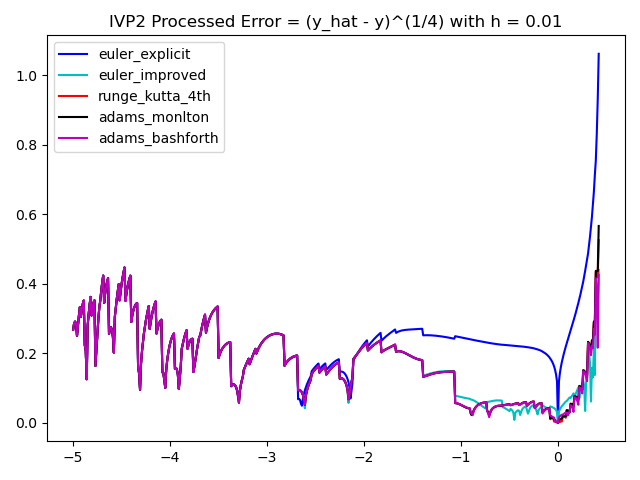
\includegraphics[width=5cm]{img/ivp2_error.png}
    		\caption{\label{fig:ivp2_error}}
    	\end{minipage}
    }
    \caption{Error Comparison Graphs of IVP1, IVP2} 
    \end{figure}

   In theoretical, for Euler Method, the global truncation error is proportional to the 1st power of h, so the error might be the largest among these methods. For improved Euler method, the global truncation error is proportional to the 2nd power of h. The fourth-order four-stage Runge-Kutta method has a global truncation error of $h^4$. The Adams-Moulton method has a global truncation error of $h^5$.
   
   From this comparison graph another conclusion come into being: it is not the case that the more accurate a method is, the better it is. Since the RK4 method has a global truncation error of $h^4$ and improved Euler method has a global truncation error of $h^3$, while they have quite close solutions. So accuracy is not the only factor we need to consider, to judge whether a method is suitable or not for one ODE, we need to consider if it is worthwhile spending much more time on calculation to increase only very small amount of accuracy. 
   
   In this case, computation complexity should also be considered.
	
	%_____________________________________________
	\subsection{Computation complexity comparison}
	
   In general, "Computation Complexity" can be composed of "Time Complexity" and "Space Complexity ". Since the two can convert to each other and in numerical methods the intermediate processes of each method mainly have effect on the total time. So time complexity will be the main part discussed here.
	
% \usepackage{booktabs}
% \usepackage{graphicx}
\begin{table}[H]
\centering
\resizebox{\textwidth}{!}{%
\begin{tabular}{@{}ccccccccc@{}}
\toprule
\textbf{h} & \textbf{Euler\_explicit} & \textbf{Eul\_implicit} & \textbf{Eur\_trape} & \textbf{Eul\_imprd} & \textbf{RK\_3rd} & \textbf{RK\_4th} & \textbf{Adams\_monlt} & \textbf{Adms\_bashforth} \\ \midrule
0.01       & 0.199389648              & 3.893579102            & 3.191479492           & 0.398876953           & 0.498486328      & 0.797802734      & 22.0447998            & 1.19675293               \\
0.005      & 0.39909668               & 6.683203125            & 6.183374023           & 0.797827148           & 1.097021484      & 1.495996094      & 43.6833252            & 2.393554688              \\
0.001      & 1.996264648              & 29.11706543            & 30.41862793           & 4.089111328           & 5.485375977      & 7.830151367      & 197.6515381           & 14.06235352              \\
0.0005     & 3.889575195              & 54.87087402            & 54.06862793           & 8.577001953           & 10.9706543       & 15.75786133      & 406.0815674           & 29.12207031              \\
0.0002     & 10.27258301              & 143.0174561            & 132.257959            & 19.64763184           & 27.33054199      & 40.19226074      & 955.9131592           & 63.23076172              \\
0.0001     & 24.43808594              & 290.3356445            & 232.636792            & 38.99562988           & 56.57814941      & 85.29304199      & 1956.909473           & 143.8662109              \\ \bottomrule
\end{tabular}%
}
\caption{Time Consuming  with different h in IVP1}
\label{tab:IVP1}
\end{table}
    
    % \usepackage{booktabs}
% \usepackage{graphicx}
\begin{table}[H]
\centering
\resizebox{\textwidth}{!}{%
\begin{tabular}{@{}ccccccccc@{}}
\toprule
\textbf{h} & \textbf{Euler\_explicit} & \textbf{Eul\_implicit} & \textbf{Eul\_trape} & \textbf{Eul\_improved} & \textbf{RK\_3rd} & \textbf{RK\_4th} & \textbf{Adams\_monlt} & \textbf{Adams\_bashforth} \\ \midrule
0.01       & 1.19260254            & 48.57026367              & 43.97243652           & 2.78720703               & 3.49047852       & 5.28737793       & 315.6517334           & 6.38789062                \\
0.005      & 2.59301758            & 59.17590332              & 48.36687012           & 5.88430176               & 7.67946777       & 10.57209473      & 443.2843994           & 13.06520996               \\
0.001      & 12.9652832            & 30.43623047              & 33.61003418           & 30.71765137              & 41.64165039      & 54.85251465      & 493.8230713           & 66.11806641               \\
0.0005     & 28.42741699           & 54.05429687              & 67.07429199           & 61.84191895              & 77.99611816      & 109.7824219      & 806.3147949           & 132.3153076               \\
0.0002     & 75.06044922           & 140.6254883              & 178.127832            & 160.380542               & 198.1198486      & 261.8647461      & 1660.448975           & 337.3976074               \\
0.0001     & 162.1139404           & 289.7324219              & 379.6040283           & 339.4297119              & 399.6322754      & 538.4823975      & 3068.49563            & 685.1721191               \\ \bottomrule
\end{tabular}%
}
\caption{Time Consuming  with different h in IVP2}
\label{tab:IVP2}
\end{table}

    The Euler method has the advantage that the formula is simple and easy to run in computer. It costs least time to finish the calculation.
    The computation complexity of the improved Euler method’s algorithm increases compared to the Euler method, since $f(t,y)$ should be evaluated twice in the formula to go from $t_n$ to $t_n+1$ in the formula.
    The fourth-order four-stage Runge-Kutta method, weighing four steps with ${1\over6}(k_{n1}+2k_{n2}+2k_{n3}+k_{n4})$. An increasing in accuracy will lead to a more complex algorithm.
    The Adams-Moulton method and the Adams-Bashforth method are multi-step methods, it would take much more time to evaluate.
    Using a "Big-O" method to evaluate these methods, the conclusion is that all methods are in the order of $O(mn)\in{O(n)}$,$m\in{O(1)}$
    
    In a certain range, there exists a negative correlation between computation complexity and accuracy. However, this is not always true. 
    
    In addition, the time consuming might also influenced by the detailed ODE functions. For IVP1, the Adams-Moulton method is most time-consuming, instead for IVP2, the Adams-Bashforth method is the most time-consuming one.

	
	%_____________________________________________
	
    \section{Conclusion}
    
	Usually a high accuracy method would cost more time and space to get the solution, however, within the tolerable margin of error, a simpler method would be more suggested.
	
	In a conclusion, every method has its own merit and demerit.	
	In reality Which one to choose should depend more on the detailed ODE function and the balance between accuracy and computation complexity requirements.
	
	%_____________________________________________
	
	
	\section{Reference List and Appendix}
	
	%插入文献
	CN DOTA, BEST DOTA!\upcite{Menard2002Applied,Peduzzi1996A,Compton2002HABITAT}
	
	
	
	
	%_____________________________________________
	
	%插入文献,IEEEtran为格式,sample为.bib文件名
	\bibliographystyle{IEEEtran}
	\bibliography{sample}
	
\end{document}